%% LyX 2.1.2 created this file.  For more info, see http://www.lyx.org/.
%% Do not edit unless you really know what you are doing.
\documentclass[english,t]{beamer}
\usepackage[T1]{fontenc}
\usepackage[utf8]{luainputenc}
\setcounter{secnumdepth}{3}
\setcounter{tocdepth}{3}
\usepackage{fixltx2e}
\usepackage{graphicx}

\makeatletter
%%%%%%%%%%%%%%%%%%%%%%%%%%%%%% Textclass specific LaTeX commands.
 % this default might be overridden by plain title style
 \newcommand\makebeamertitle{\frame{\maketitle}}%
 % (ERT) argument for the TOC
 \AtBeginDocument{%
   \let\origtableofcontents=\tableofcontents
   \def\tableofcontents{\@ifnextchar[{\origtableofcontents}{\gobbletableofcontents}}
   \def\gobbletableofcontents#1{\origtableofcontents}
 }

\@ifundefined{date}{}{\date{}}
%%%%%%%%%%%%%%%%%%%%%%%%%%%%%% User specified LaTeX commands.
\usetheme{rwth}
\usepackage{braket}

\title{Polarimetry concepts for the EDM precursor experiment at COSY}
\subtitle{\vspace{2cm} \hspace{15cm} 
\includegraphics{gfx/jedi_logo2.png} \vspace{-2cm}}
\author{Paul Maanen}
\institute{Physics Institute III B, RWTH Aachen University}
\date[\today]{DPG Frühjahrstagung \today}

% Some changes on the layout, can be switched off by commenting out
\setheadlinestyle{headlineframetitle}
\setfooterstyle{footertitleauthor}
\setfootlinestyle{footlinedatepages}

% German style date formatting (footer)
\usepackage[ddmmyyyy]{datetime}
\renewcommand{\dateseparator}{.}

% To get greek letters better matching with rest of font
\usepackage{upgreek}

\logo{
\includegraphics{gfx/rwth_3physik_b_englisch_rgb.png}}

\makeatother

\usepackage{babel}
\begin{document}
\setbeamercolor{title page bar}{fg=rwth} 
\setbeamertemplate{title page}[rwth]{} 
\begin{frame}[plain]{}


\titlepage
\end{frame}

\begin{frame}{Outline}


\tableofcontents{}

\end{frame}



\section{Motivation}
\begin{frame}{Design goals for an EDM polarimeter}

\begin{itemize}
\item Current candidate method for EDM search implicates a linear buildup
of polarization with time.
\item Design goals for polarimeter:

\begin{itemize}
\item High $\sigma_{el}$,$A_{y}$
\item Minimal influence on beam
\item Low sensitivity to systematic effects
\end{itemize}
\end{itemize}

\end{frame}



\section{Detector concept}
\begin{frame}{Target choice}

\begin{itemize}
\item Carbon was chosen as best overall target choice
\item Big cross section and analysing power, easy to handle
\item XSec, Ay, FOM 50, 250 MeV
\end{itemize}

\end{frame}

\begin{frame}{Target concept}


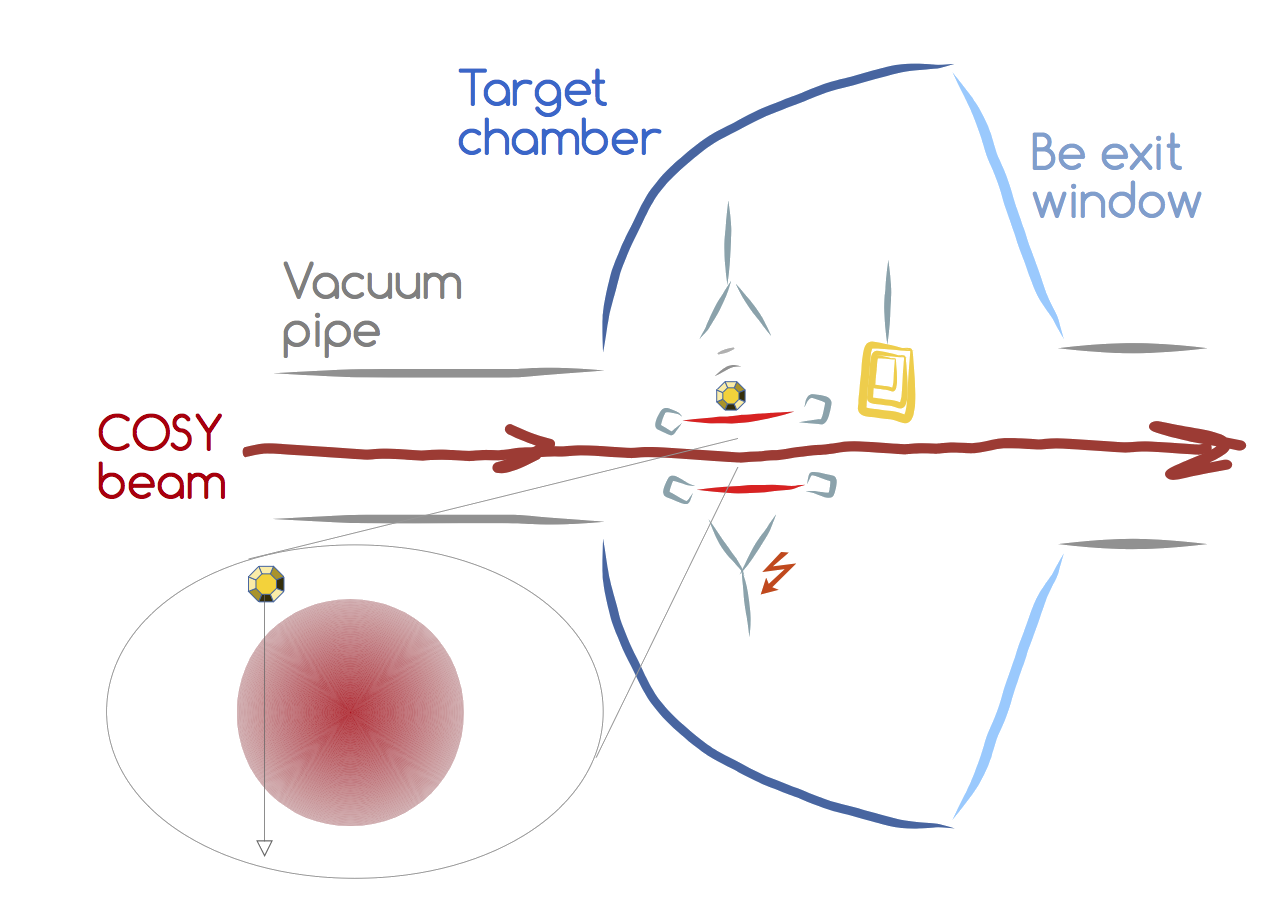
\includegraphics[height=1\textheight]{gfx/target}




\end{frame}

\begin{frame}{Detector concept}


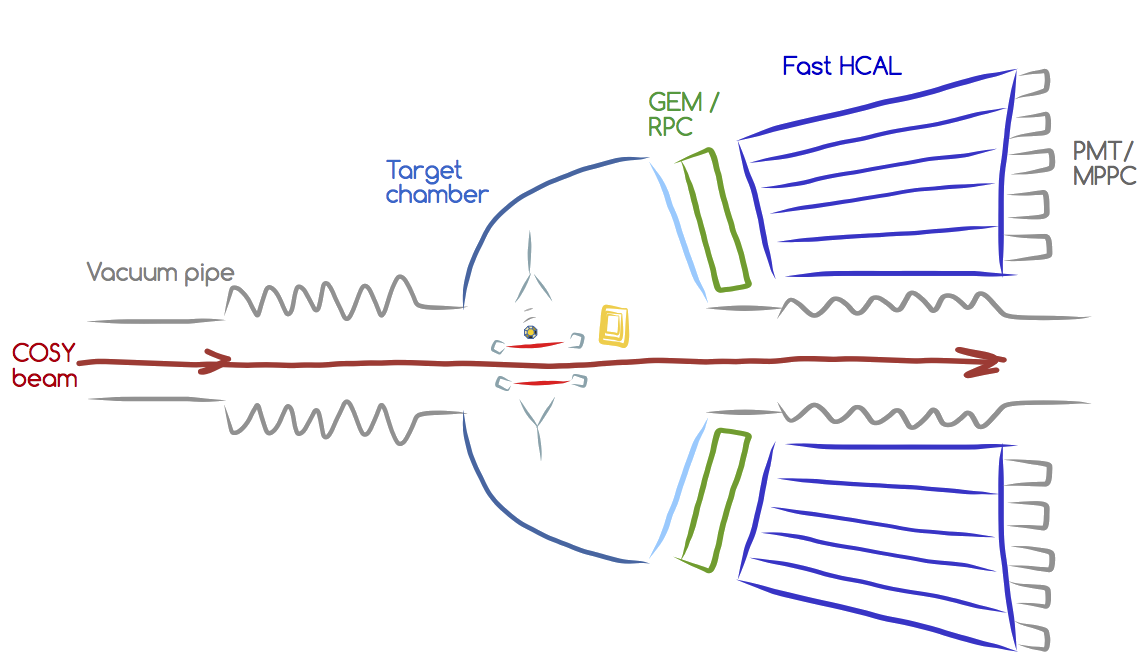
\includegraphics[height=1\textheight]{gfx/detector}

\end{frame}

\begin{frame}{Readout Concept}


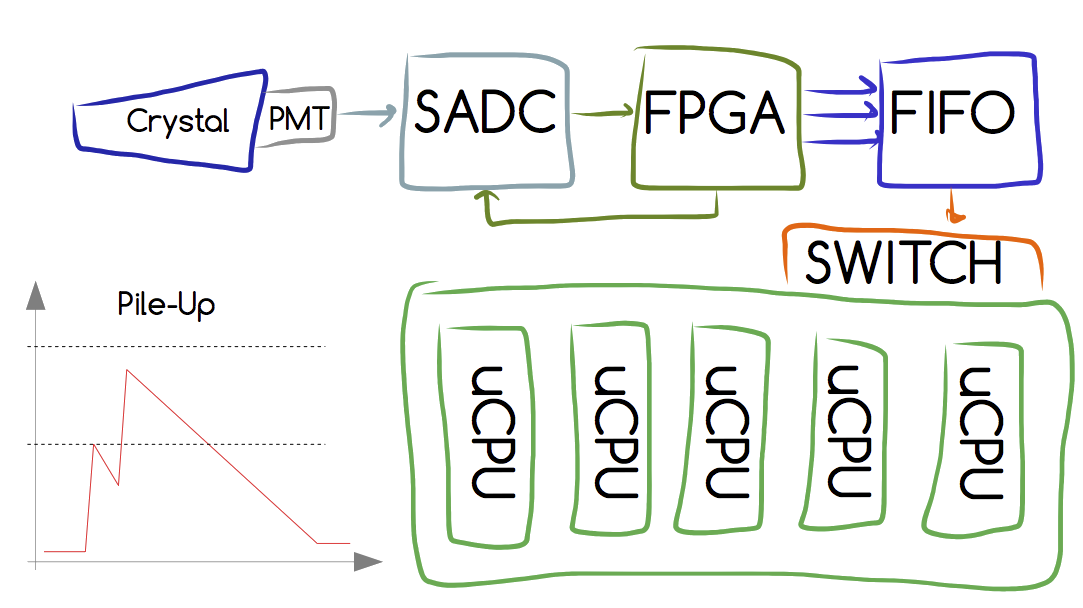
\includegraphics[height=0.8\textheight]{gfx/readout}
\begin{itemize}
\item Triggerless readout: Use waveform digitizers and read out every turn.
\item Use FPGA-based online analysis
\end{itemize}
\end{frame}

\begin{frame}{Readout Concept (cont'd)}


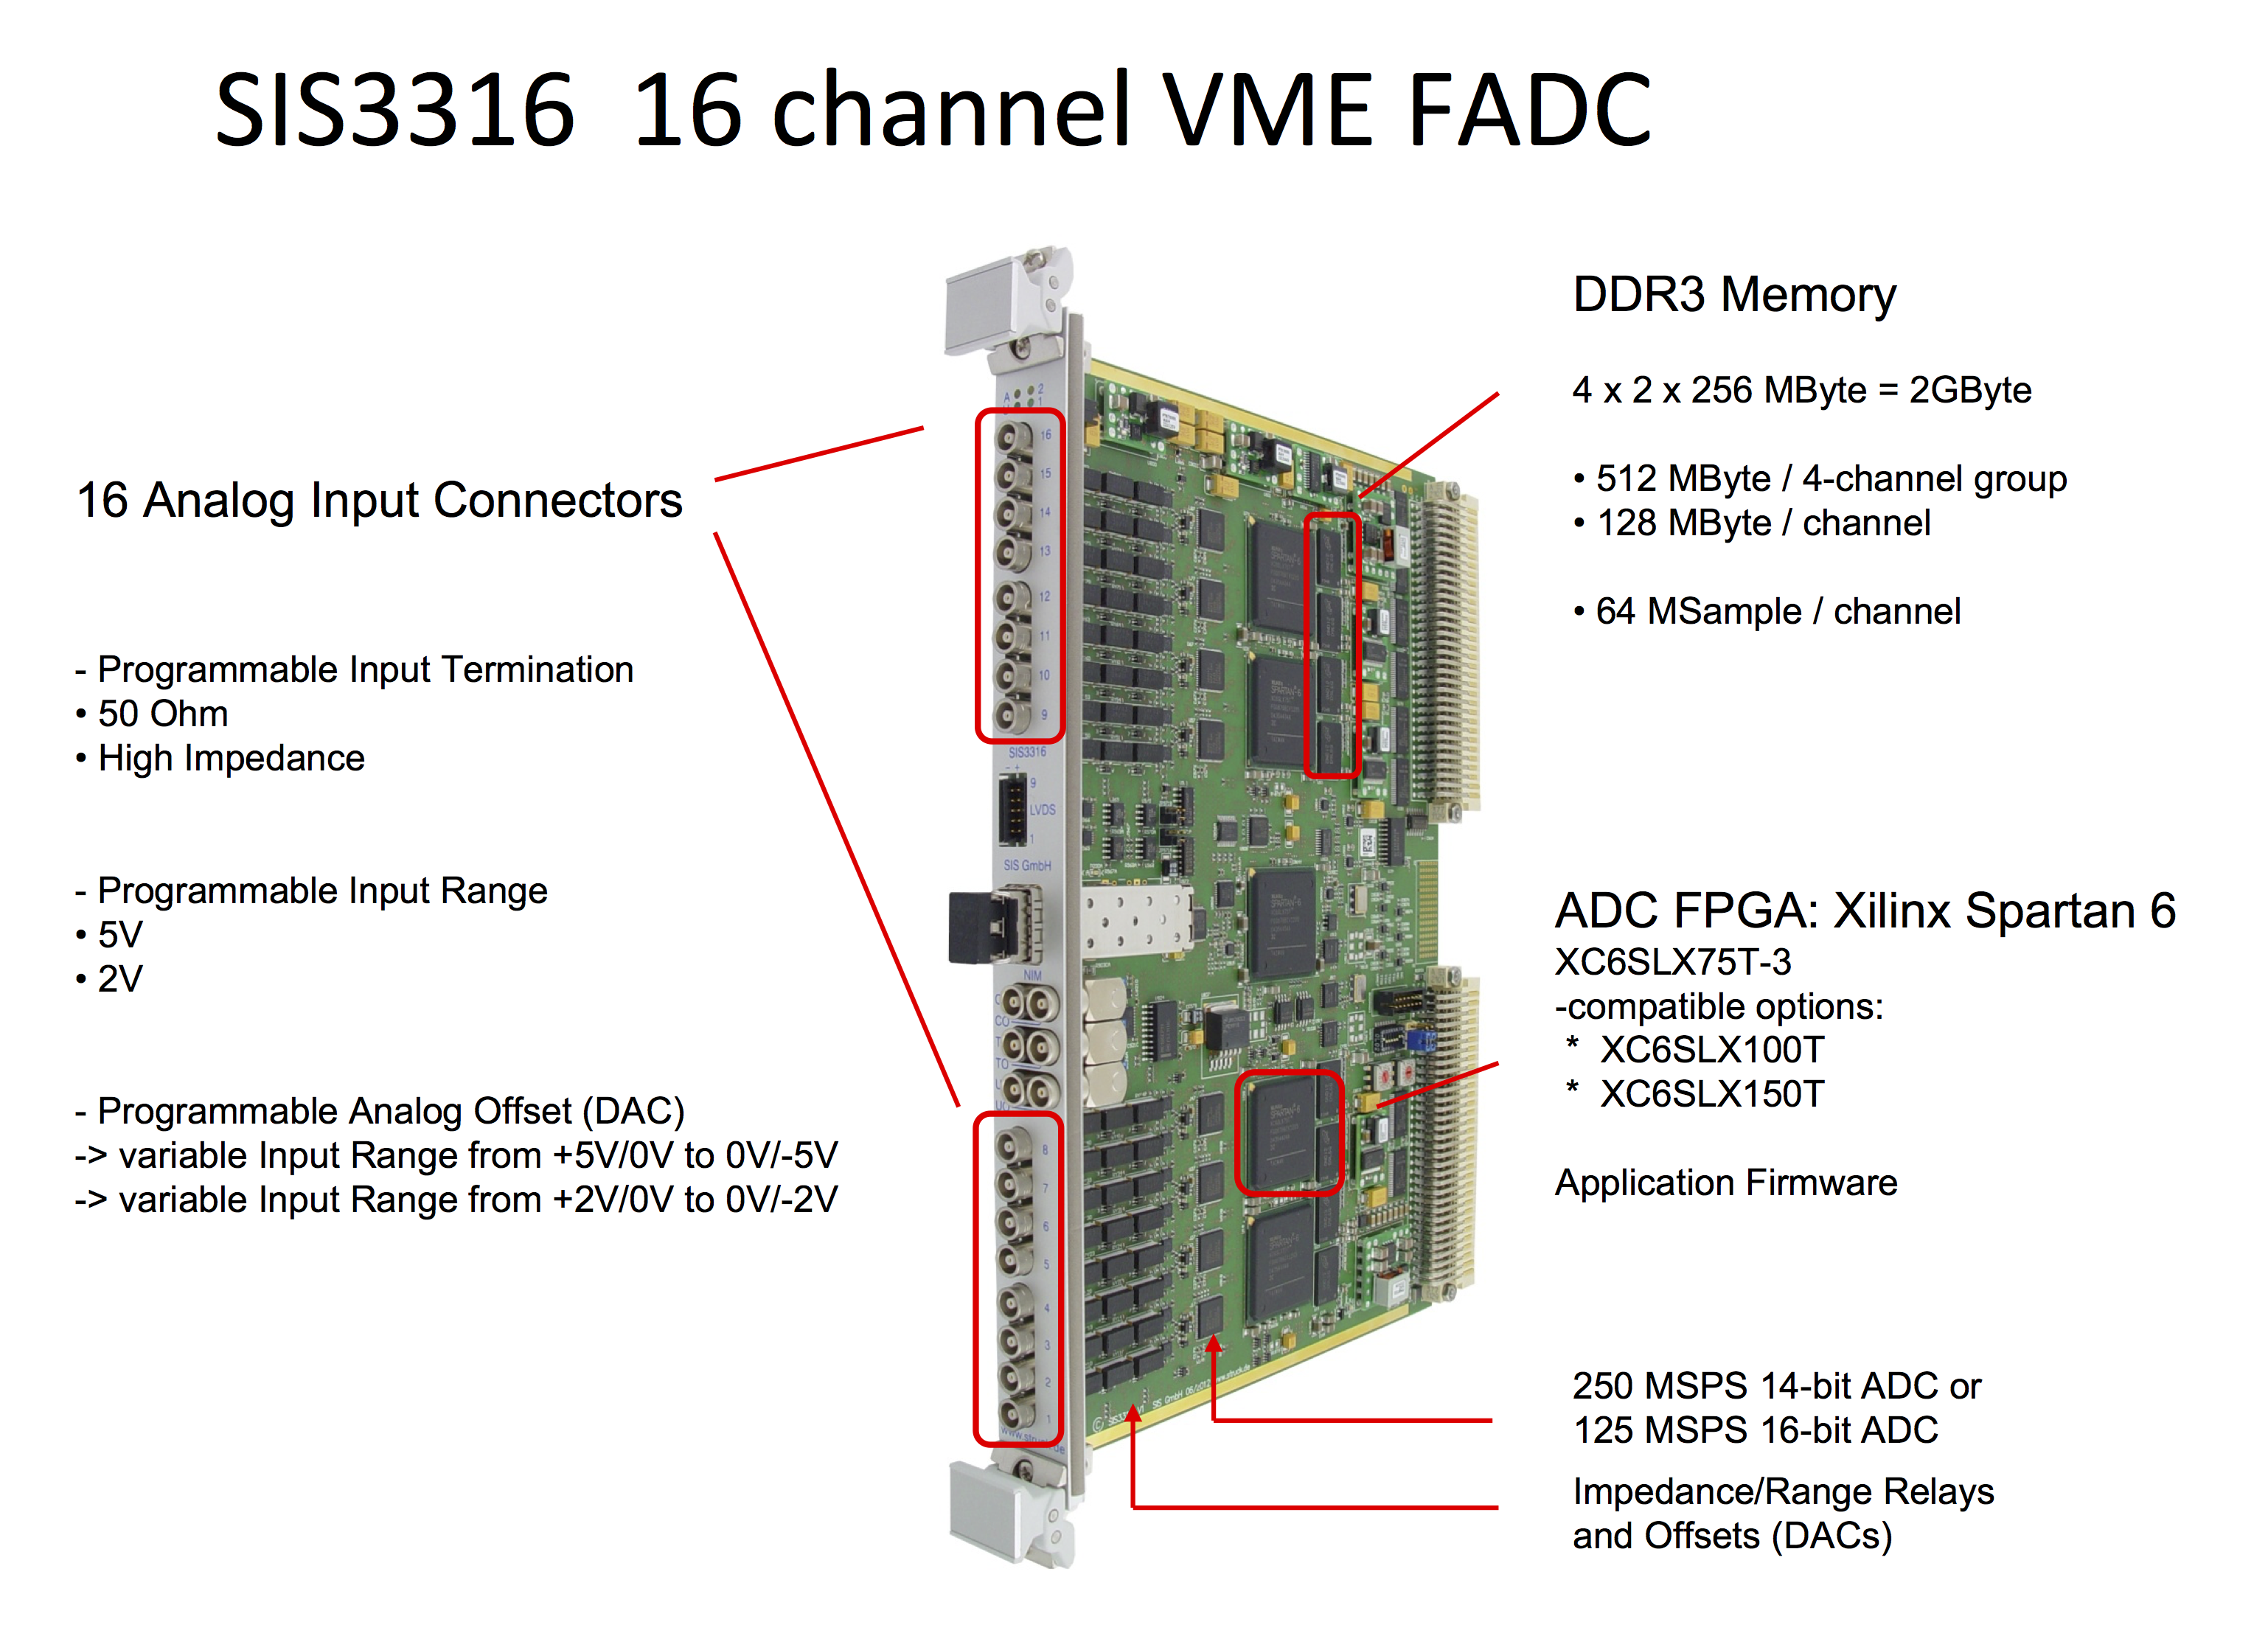
\includegraphics[height=1\textheight]{gfx/sis}


\end{frame}

\section{Detector}
\begin{frame}{Candidate Layout}

\end{frame}

\begin{frame}{Simulation studies}


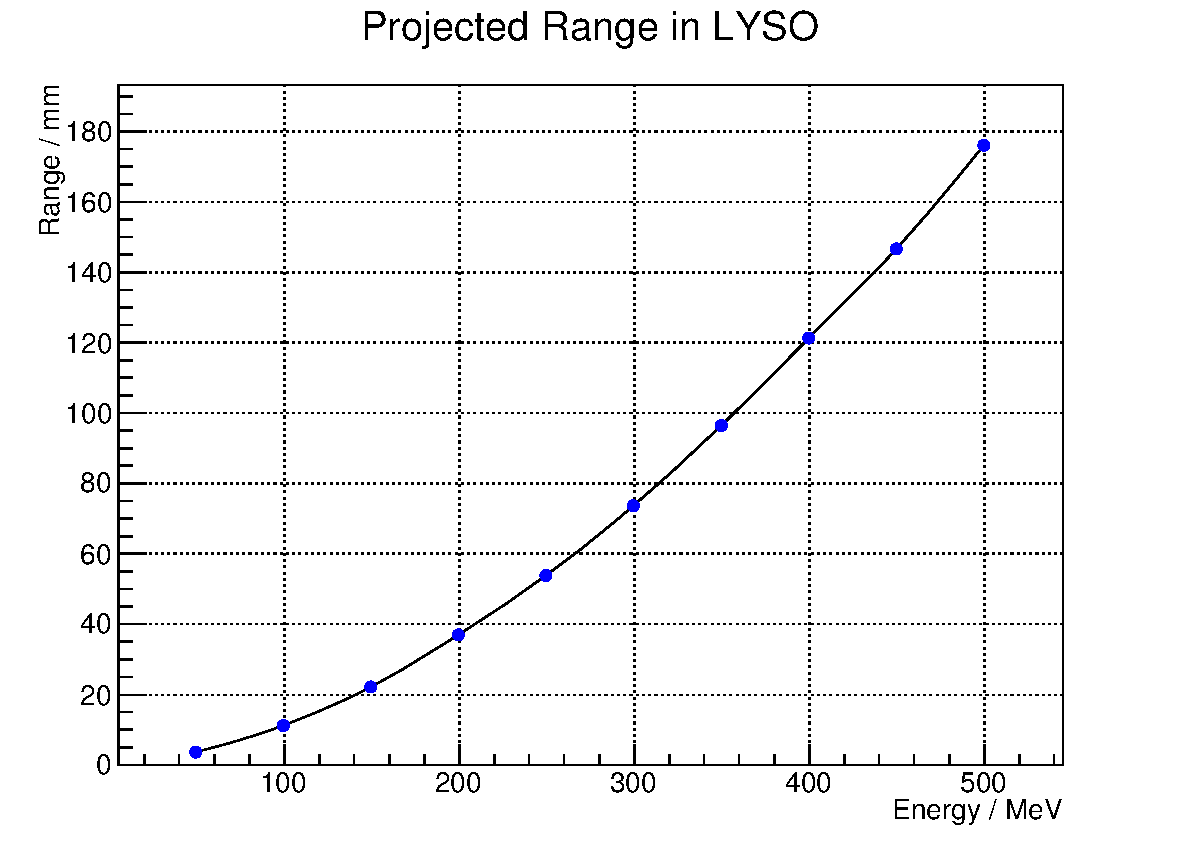
\includegraphics[width=0.75\paperwidth]{gfx/LYSO}


\end{frame}

\begin{frame}{Simulation studies (cont'd)}

\begin{itemize}
\item Lyso vs Plastic+Degrader vs Sandwich
\end{itemize}

\end{frame}

\section{Summary \& Outlook}
\begin{frame}{Summary \& Outlook}

\begin{itemize}
\item Have a candidate layout for JEDI polarimeter
\item Crystals have been ordered for hardware tests.
\item Will explore gain from tracking capabilities.
\item New student will begin work on target end of year.\end{itemize}
\end{frame}

\end{document}
